
This work relies on optimal control theory and orbital mechanics. Certain tools from optimal control theory are necessary to analyze the conditions for a control trajectory to be the best according to some criterion, and under some mathematical conditions. This theory applies to a wide range of linear and non-linear systems, independently of the specifics of a dynamical system. However, this works focuses its application to one particular system: that of a body gravitationally attracted by a much more massive central body, which is the domain of orbital mechanics. Both theories will be introduced in the following sections.

\section{Optimal Control}

Optimal control is the area of control theory which tries to find the best control action to satisfy some requirements, such as altering a system's state in some desired way. Here, ``best''  is defined as maximizing or minimizing some performance metric. In practice, and in particular in the scope of this work, this can be interpreted as attaining a target orbit in a certain amount of time, while minimizing fuel consumption.

The mathematical nature of an optimal control problem varies greatly depending on the nature of the system, the requirements, and the objective. Here, a selected subset of this vast theory shall be presented. Suppose a continuous time dynamical system operating on times \(t \in [0, t_f]\), where \(t_f \in \mathbb{R}\), given by

\begin{equation} \label{eq:generic_dyn}
    \dot{\mathbf{x}}(t) = f(\mathbf{x}(t), \mathbf{u}(t))
\end{equation}
where \(\mathbf{x}(t): \mathbb{R} \rightarrow \mathcal{\mathbf{x}} \subset \mathbb{R}^n\) is the state vector trajectory describing the system state, \(\mathbf{u}(t): \mathbb{R} \rightarrow \mathbb{R}^m\) is the control vector trajectory and \(f: \mathbb{R}^n \times \mathbb{R}^m \rightarrow \mathbb{R}^n\) is the function describing its temporal dynamics. Those functions are supposed to belong to function spaces with certain regularity properties, which will be discussed in Section~\ref{sec:imp_prop_model} in the context of impulsive control.

In addition, the control vector might be subject to some some inequality constraints, representing for instance saturation of actuators. Therefore, an admissible control set \(\mathcal{U}\) is defined by a vector of constraint functions \(\mathbf{g}(\mathbf{u})\) as
\begin{equation}
    \mathcal{U} = \left\{\mathbf{u} \in \mathbb{R}^m |\; \mathbf{g}(\mathbf{u}) \leq 0\right\}
\end{equation}
where the inequality is understood to hold component-wise.

At the initial time, the system is supposed to be in a given state \(\mathbf{x}_i\) such that 
\begin{equation} \label{eq:generic_initial_constraint}
    \mathbf{x}(0) = \mathbf{x}_i.
\end{equation}

At the final time \(t_f\), some components of the final state vector are specified, while others are subject to optimization. Let the index set \(\mathcal{K}\) be the set of state variables that are fixed at the final time, such that
\begin{equation} \label{eq:generic_final_constraint}
    (\mathbf{x}(t_f))_k = (\mathbf{x}_{f})_k, k\in \mathcal{K},
\end{equation}
where \(\mathbf{x}^k\) denotes the k-th component of \(\mathbf{x}\), for some given values \(\mathbf{x}_{f}^k\).

To complete the optimal control problem, a performance metric needs to be introduced. In general, any functional of the form \(J[\mathbf{x}(t), \mathbf{u}(t)]\) may be taken as this performance metric; however, a common form which shall be adopted in this work, is given by
\begin{equation} \label{eq:generic_cost}
    J[\mathbf{x}(t), \mathbf{u}(t)] = h(\mathbf{x}(t_f)) + \int_0^{t_f} L(\mathbf{x}(t), \mathbf{u}(t)) dt
\end{equation}
where the functions \(h(\mathbf{x})\) and \(L(\mathbf{x}, \mathbf{u})\) are respectively called the \textit{terminal cost} and the \textit{temporal cost} functions~\cite{bertsekas}.\

The optimal control problem is then that of finding a control trajectory \(\mathbf{u}(t)\) that minimizes (or maximizes) the performance metric. Here the problem shall be presented as a minimization problem; but the formulation is perfectly analogous for a maximization problem. That said, the complete optimal control problem may be stated as finding the function \(\mathbf{u}(t)\) such that~\cite{bryson_applied_optimal_control}

\begin{equation} \label{eq:argmin_cost}
    \mathbf{u}(t) = \arg \min_{\mathbf{u}(t), \mathbf{x}(t)} J[\mathbf{x}(t), \mathbf{u}(t)]
\end{equation}
subject to
\begin{align}
    \dot{\mathbf{x}}(t) &= f(\mathbf{x}(t), \mathbf{u}(t)) \\
    \mathbf{x}(0) &= \mathbf{x}_i \\
    \left(\mathbf{x}(t_f)\right)_k &= (\mathbf{x}_f)_k, k\in \mathcal{K}.
\end{align}

In general, this is a very hard problem. The optimization variables \(\mathbf{u}\) and \(\x\) are infinite dimensional. There are techniques to turn this problem into a simple parameter optimization problem, which are known as \textit{direct methods}~\cite{Conway_2010}, which shall be discussed later. There are however tools for extracting necessary conditions for the optimal solution of this problem at all points in time. These are known as \textit{indirect methods}.

One of this tools is the Hamiltonian~\cite{Conway_2010}, a quantity that describes the ensemble of objectives and constraints. It shall be defined for a minimization problem, and maximization problems can be adapted by changing the sign of the performance metric. Given a system of the form in Equation~\eqref{eq:generic_dyn}, constraints in the forms of Equations~\eqref{eq:generic_initial_constraint} and~\eqref{eq:generic_final_constraint}, and a cost function in the form~\eqref{eq:generic_cost}, the Hamiltonian \(H\) is defined as~\cite{bertsekas}
\begin{equation}
    H(\mathbf{x}(t), \mathbf{u}(t), \mathbf{\lambda}(t)) = L(\mathbf{x}, \mathbf{u}) + \mathbf{\lambda}{(t)}^T f(\mathbf{x}, \mathbf{u})
\end{equation}
for all times \(t\), state and control vectors \(\mathbf{x}  \) and \(\mathbf{u}\) along a trajectory.\ \( \mathbf{\lambda}: \R \rightarrow \R^n, \mathbf{\lambda} \in C^1\) is the costate trajectory, a new set of variables introduced as the continuous-time equivalent of Lagrangian multipliers. These new variables are subject to the adjoint equations
\begin{equation}
    \dot{\mathbf{\lambda}} = - \left( \frac{\partial H}{\partial \mathbf{x}} \right)^T = -\left( \frac{\partial f}{\partial \mathbf{x}} \right)^T \mathbf{\lambda} - \left( \frac{\partial L}{\partial \mathbf{x}} \right)^T
\end{equation}
and boundary conditions~\cite{bryson_applied_optimal_control}
\begin{equation}\label{eq:final_costate}
    \mathbf{\lambda}^k(t_f) = \frac{\partial h(\mathbf{x}(t_f))}{\partial \mathbf{x}^k}, k \notin \mathcal{K}.
\end{equation}

An important property of the Hamiltonian for fixed-time problems is that its value is constant with respect to time along the optimal trajectory~\cite{bertsekas}. For an optimal trajectory \(\x^\star(t)\), \(\uc^\star(t)\), \(\lambda^\star(t)\), and some value \(C \in \R\),
\begin{equation}\label{eq:constant_hamilt}
    H(\x^\star(t), \uc^\star(t), \lambda^\star(t)) = C, \forall t \in [0, t_f].
\end{equation}

To complete the Hamiltonian approach, Pontryagin's Minimum Principle (PMP) is introduced. It states that a necessary condition for attaining the minimum in Equation~\eqref{eq:argmin_cost} is that, at all times \(t\), and along the optimal trajectory,~\cite{bertsekas}
\begin{equation} \label{eq:Pontryagin}
    \mathbf{u}^\star(t) = \arg \min_{\mathbf{u} \in \mathcal{U}} H[\mathbf{x}(t), \mathbf{u}, \mathbf{\lambda}(t)].
\end{equation}

With the control trajectory obtained as a function of \(\mathbf{x}(t)\) and \(\mathbf{\lambda}(t)\) from Equation~\eqref{eq:Pontryagin}, there are 2n variables, the state and costate trajectories, and 2n boundary conditions, the initial states, some final states and some final costates according to Equations \eqref{eq:generic_final_constraint} and \eqref{eq:final_costate}. Thus, the problem is well-posed and configures a Two Point Boundary Value Problem (TPBVP)~\cite{bryson_applied_optimal_control}.

It is worth highlighting that in optimal control problems, a hierarchy of solutions exist~\cite{ross2015primer}, shown in Figure~\ref{fig:opt_sol_hierarchy}. The least valuable solution is a mere feasible solution, which satisfies the constraints, but is not optimal in any sense. It is enough in some applications, but not in others. Next, local optima have generally lower costs, and are found numerically with nonlinear solvers, but no not necessarily reflect extrema of the original problem. If it can be shown that a local optimum also satisfies the PMP, it comes is inherently a more valuable solution, since it satisfies the necessary conditions to be an extremum of the problem. The most valuable solution type, and the one which is almost impossible to characterize, are global optima, which are guaranteed to have the lowest possible feasible cost for the problem. Finally, lower bound estimations give (infeasible) costs which are guaranteed to be lower than the global optimum, and can be estimated physically~\cite{impulsive_europa} or mathematically, for instance with sum-of-squares decompositions~\cite{sos_book}. This work will search for extrema satisfying the PMP.

\begin{figure}[htbp]
    \centering
    \begin{tikzpicture}
        \node (feas) [process] {Feasible solution};
        \coordinate [left=of feas] (feas_left);
        \node (loc) [process, below=of feas] {Local optimum};
        \node (ext) [process, below=of loc] {Extremum satisfying PMP};
        \node (global) [process, below=of ext] {Global optimum};
        \node (lb) [startstop, below=of global] {Lower bound};
        \coordinate [left=of lb] (lb_left);
        \draw [arrow] (feas_left) node[left=3mm] {Decreasing cost}-- (lb_left);
    \end{tikzpicture}
    \caption{Hierarchy of optimal control problem solutions. Adapted from~\citeonline{ross2015primer}.}
    \label{fig:opt_sol_hierarchy}
\end{figure}


TODO: NUMERICAL APPROACH: MULTIPLE SHOOTING


\section{Orbital Mechanics}

Orbital mechanics concerns itself with the motion of bodies in space subject to gravitational and disturbance forces. A variety of models exist, differing in precision and availability of analytical tools. The simpler the model, the more analytical tools are available, and the smaller the precision. The simplest model of all, and the basis for all others, is the two body problem, where a central massive body is supposed to be stationary while a moving satellite is subject to its gravitational attraction, also known as Keplerian motion. 

\subsection{Two Body Motion}

Let \(\mathbf{r}\) be the 3-dimensional position of a satellite, and \(\mu \) the gravitational parameter of the central body. The dynamics of the satellite's position are given by~\cite{curtis2015orbital}
\begin{equation} \label{eq:kepler_dyn}
    \ddot{\mathbf{r}} = g(\mathbf{r}) = -\frac{\mu}{\lVert \mathbf{r} \rVert^3} \mathbf{r},
\end{equation}
where \(g(\mathbf{r})\) represents the gravitational acceleration field, thus configuring a 6-dimensional state vector \(\mathbf{x} = \begin{bmatrix}
    \mathbf{r}^T & \mathbf{v}^T
\end{bmatrix}^T\), where \(\mathbf{v}\) is the satellite's velocity. The system contains a singularity at the states with \(\lVert \mathbf{r} \rVert = 0\), which configures a non-convex domain. In practice, this point is rarely encountered as it lies inside of the central body, thus far from the regions of interest. It is proven that no analytical solution exists for this differential equation; however, much is known about its solutions.

In this model, the possible trajectories are known to be conics, and therefore restricted to a plane. For bound satellites, that is, those in orbit around the central body, this trajectory is an ellipse where the central body lies on one of its foci. Mathematically, a ``bound'' satellite is one whose specific energy (mechanical energy over mass of the satellite), given by~\cite{curtis2015orbital}
\begin{equation}
    \epsilon = -\frac{\mu}{\lVert \mathbf{r} \rVert} + \frac{\mathbf{v}^2}{2},
\end{equation}
is negative. The trajectory is closed, and the movement is periodic with period~\cite{curtis2015orbital}
\begin{equation}
    T = 2\pi \sqrt{\frac{a^3}{\mu}}
\end{equation}
where \(a\) is the semi-major axis of the ellipse.

In this case, an alternative state vector may be introduced in the form of the Keplerian elements. These are~\cite{curtis2015orbital}:
\begin{itemize}
    \item \(a\): semi-major axis of the ellipse;
    \item \(e\): excentricity of the ellipse;
    \item \(i\): inclination of the orbit's plane with respect to the equatorial plane;
    \item \(\Omega \): right ascension of the ascending node, that is, angle between the vernal equinox direction and the direction where the satellite crosses the equatorial plane from South to North;
    \item \(\omega \): argument of perigee, or angle, in the plane of the orbit, between the ascending node and the perigee (point of smallest distance to the central body);
    \item \(\theta \): true anomaly, or angle between the perigee and the current position of the satellite.
\end{itemize}

These elements are related to the Cartesian state vector through the geometric description of a point on an ellipse, rotated through the Euler angles \(\Omega\), \(i\), \(\omega\)~\cite{curtis2015orbital}.


In this formulation, only the true anomaly is a function of time, all other elements being constant. The true anomaly can be related to time implictly through two other quantities, the mean anomaly \(M\) and the excentric anomaly \(E\)~\cite{curtis2015orbital}:

\begin{align} 
        M &= 2\pi \frac{t - t_p}{T} \\
        E - e \sin{E} &= M \label{eq:kepler_equation}\\
        \tan{\frac{\theta}{2}} &= \sqrt{\frac{1+e}{1-e}} \tan{\frac{E}{2}} \label{eq:true_exc_anom}
\end{align}
where \(t_p\) is the time of the last perigee passage. By computing the mean anomalies in an initial and a final time, and solving the notorious Kepler's Equation~\eqref{eq:kepler_equation}, and finally finding a suitable true anomaly with Equation~\eqref{eq:true_exc_anom}, a semi-analytical temporal solution can be found. The process of finding the position of a satellite in the future is called \textit{orbit propagation}. Define an orbit propagator as a funcion \(p_o(\mathbf{x}_i, t)\) such that
\begin{equation} \label{eq:orbit_propagator}
    \mathbf{x}_f = p_o(\mathbf{x}_i, t)
\end{equation}
where \(\mathbf{x}_f\) is the satellite's final state after a time \(t\), with initial state \(\mathbf{x}_i\).

\subsection{Orbital Perturbations}

The two body model is an idealized model amenable to analytical solutions, which neglects many real world phenomena. In LEO, the most important perturbations are oblateness effects (J2) and atmospheric drag~\cite{curtis2015orbital}, which are introduced ahead.

\subsubsection{Oblateness effects}

The Earth being an oblate spheroid, its gravity field is not perfectly central, neither does it behave like the inverse square law predicted by the two body model. Instead, the Earth's geopotential is modeled as a point mass potential plus spherical harmonics terms with coefficients subject to empirical fitting. The biggest non-sphericity of Earth is its oblateness, the increased width at the Equator. This effect is described by the coefficient \(J_2\), which causes a perturbing acceleration \(\mathbf{a}_{J2}\) given by
\begin{equation}\label{eq:j2_acc}
    \mathbf{a}_{J2} = \frac{3 J_2 \mu R^2}{2 r^4} \begin{bmatrix}
        \frac{x}{r} \left(5 \frac{z^2}{r^2} - 1\right) \\
        \frac{y}{r} \left(5 \frac{z^2}{r^2} - 1\right) \\
        \frac{z}{r} \left(5 \frac{z^2}{r^2} - 3\right)
    \end{bmatrix},
\end{equation}
where \(R\) is Earth's Equatorial radius.

Thus, this model's dynamics can be expressed solely as a function of the position, since it is a conservative model:
\begin{equation}
    \ddot{\mathbf{r}} = g_{J2}(\mathbf{r}) = -\frac{\mu}{r^3} \mathbf{r} + \mathbf{a}_{J2}.
\end{equation}

\subsubsection{Atmospheric Drag}\label{sssec:drag}

Atmospheric drag affects satellites in LEO by generating a force opposed to the relative velocity of the satellite w.r.t.\ the Earth's atmosphere, which rotates with it. The drag force is proportional to atmospheric density \(\rho(r)\), as a function of the satellite's distance to Earth. Modelling this dependence is not a trivial task, with accurate models taking solar activity and Earth's temperature into account. A simple model is given by the US Standard Atmosphere 1976, which gives empirical coefficients \(\rho_i\) and \(H_i\), valid for height intervals \([h_i, h_i+1]\), for \(i = 1,\dots, 28\). Then, atmospheric density is given piecewise by
\begin{equation}\label{eq:rho}
    \rho(r) = \rho_i \exp{\big(-\frac{\left(r - (h_i + R)\right)}{H_i}\big)},
\end{equation}
where \(i\) is such that \(h_i \leq r - R \leq h_{i+1}\). The satellite is parameterized by a reference surface \(S\), drag coefficient \(C_D\) and mass \(m\). Considering that the Earth rotates with angular velocity \(\omega_E\), the relative velocity of the satellite w.r.t.\ the atmosphere is given by
\begin{equation}
    \vel_{r} = \vel - (\omega_E \hat{\mathbf{z}}) \times \pos.
\end{equation}

Finally, the acceleration due to drag \(\acc_D\) is given by
\begin{equation}\label{eq:acc_drag}
    \acc_D = - \frac{1}{2} \rho(r) \frac{S C_D}{m} \lVert \vel_r \rVert \vel_r,
\end{equation}

which can be added as a perturbing non-conservative acceleration to the model.

\subsection{Lambert's Problem}

An important problem in orbital mechanics is that of the determination of the initial and final velocities of a satellite that passes through two points in space \(\mathbf{r}_1\) and \(\mathbf{r}_2\) with a time interval \(\Delta t\) in between, as illustrated in Figure~\ref{fig:lambert_diagram}. This problem first arose in the field of orbit determination but also finds application in the context of orbital maneuvers. Namely, Lambert's Problem seeks to find a feasible solution to a TPBVP, which is of interest to the optimal control TPBVP. 

\begin{figure}[htbp]
    \centering
    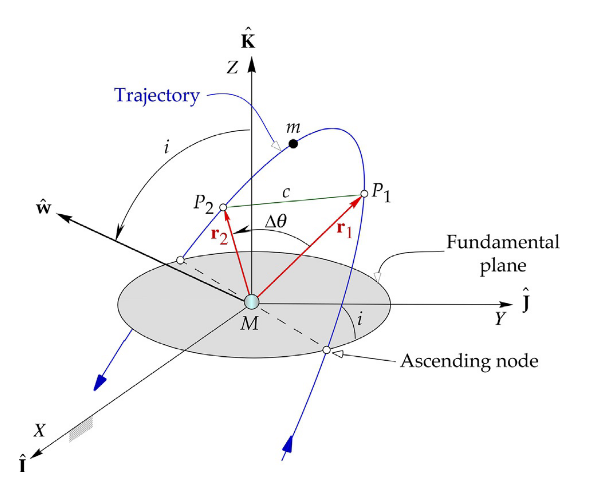
\includegraphics[width=0.6\textwidth]{img/lambert_from_curtis.png}
    \caption{Lambert problem illustration showing initial and final positions \(\mathbf{r}_1\) and \(\mathbf{r}_2\) and the (computed) trajectory that connects them in time \(\Delta t\). Source: \cite{curtis2015orbital}}
    \label{fig:lambert_diagram}
\end{figure}

This problem suffers from a physical indetermination in the case of collinear \(r_1\) and \(r_2\): the plane of the orbit is indeterminate. In this case, one can find many feasible solutions but determining exact velocities requires extra information about the plane of the orbit.\

In general, this problem can have multiple solutions, corresponding to prograde and retrograde trajectories, with less than one or multiple revolutions. The resulting orbit can, in general, be elliptic, parabolic or hyperbolic. Handling this variety of solution types is not simple. A simple formulation which does not handle multiple revolutions nor the indetermination mentioned can be built with universal variables~\cite{curtis2015orbital}. Multiple revolutions and finding the radial and tangent components of the velocity in the indeterminate case can be handled with more complex algorithms~\cite{sukhanov}. A generic, Cartesian coordinates-based algorithm is also possible, as will be discussed in Chapter~\ref{chap:method}.

\subsection{State Transition Matrix}

It is sometimes useful to characterize how the solution of an ODE depends on its initial condition. For the solution \(\x(t) \in \R^n\) of the dynamical system \(\dot{\x} = f(\x)\) with initial condition \(\x_0\), this is mathematically described by the state transition matrix (STM) \(\Phi_\delta(t) \in \R^{n \times n}\):
\begin{equation}\label{eq:stm_def}
    \Phi_\delta(t) = \frac{\partial \x(t)}{\x_0}.
\end{equation}

In general, this matrix is subject to the initial value problem~\cite{montenbruck2000satellite}
\begin{equation}
    \begin{cases}
        \dot{\Phi}_\delta(t) = \frac{\partial f(\x(t))}{\partial x(t)} \Phi_\delta(t) \\
        \Phi_\delta(0) = \mathbf{I}_n
    \end{cases}
\end{equation}
with \(n^2\) variables and initial conditions.

In particular, for a double-integrator system with position \(\pos\) and velocity \(\vel\) in the state vector described by
\begin{equation}
    \dot{\x} = \begin{bmatrix}
        \dot{\pos} \\ \dot{\vel}
    \end{bmatrix} = \begin{bmatrix}
        \vel \\ \acc(\pos, \vel)
    \end{bmatrix},
\end{equation}
the STM equation can be expanded to
\begin{equation}\label{eq:STM_r_v}
    \dot{\Phi}_\delta(t) = \begin{bmatrix}
        \mathbf{0}_{3\times 3} & \mathbf{I}_3 \\
        \frac{\partial \acc(\pos(t), \vel(t))}{\partial \pos} & \frac{\partial \acc(\pos(t), \vel(t))}{\partial \vel}
    \end{bmatrix} \Phi_\delta(t) = A_\delta(\pos(t), \vel(t)) \Phi_\delta(t),
\end{equation}
where \(A_\delta(\pos(t), \vel(t))\) is defined to be matrix coefficient of the STM in its differential equation. Note also that any vector ODE with state \(\mathbf{z}(t) \in \R^n\) subject to
\begin{equation}
    \dot{\mathbf{z}}(t) = A_\delta(\pos(t), \vel(t)) \mathbf{z}(t),
\end{equation}
its solution is given in terms of the initial condition \(\mathbf{z}_0\) and the STM:
\begin{equation}\label{eq:remark_STM}
    \mathbf{z}(t) = \Phi_\delta(t) \mathbf{z}_0.
\end{equation}

For a two-body model, an analytical expression for the STM exists, given for instance in \citeonline{montenbruck2000satellite} and \citeonline{glandorf_transition_matrix}. 

\section{Orbital Maneuvers}

When a satellite is able to maneuver, the Keplerian dynamics of Equation~\eqref{eq:kepler_dyn} need to be augmented with the thrust control vector \(\mathbf{F}\), which applies a propulsion force on the satellite. Supposing that \(m\) is the total current mass of the spacecraft, which in general is a seventh state variable (in addition to orbital state variables), the dynamics are given by
\begin{equation}
    \ddot{\mathbf{r}} = -\frac{\mu}{\lvert \mathbf{r} \rVert^3}\mathbf{r} + \frac{\mathbf{F}}{m}.
\end{equation}

The generation of thrust \(\mathbf{F}\) is tied to the consumption of propellant, according to some propulsion model. Three main models exist. The first is the constant specific impulse continuous (as opposed to instantaneous) thrust model, adequate for chemical engines. The second is the impulsive thrust model, the limiting case of the previous model where a burn is considered to happen instantly. And the last one is the continuous thrust variable specific impulse model, which models electric rocket engines and shall not be explored in this work.

The application of optimal control to the field of orbital maneuvering is mainly concerned with the preservation of propellant. Suppose a satellite has an orbital state \(\mathbf{x}_i\) and is required to maneuver to an orbital state \(\mathbf{x}_f\) in a time \(t_f\), and it is desired to minimize the amount of propellant used. A convenient way of expressing this is to maximize the final mass of the spacecraft, with constraints:
\begin{align}
    \max_{\mathbf{F}(t)}&\quad m(t_f) \label{eq:max_final_mass} \\
    \mathbf{x}(0) &= \mathbf{x}_i \\
    \mathbf{x}(t_f) &= \mathbf{x}_f
\end{align}

\subsection{Constant specific impulse model}

Chemical and cold gas thrusters are characterized by an exhaust velocity \(v_e\) at which the propellant flow is ejected from the spacecraft. With a propellant flow rate \(\dot{m}_p\), the thrust \(\mathbf{F}\) is given by
\begin{equation}
   \lVert \mathbf{F} \rVert = v_e \dot{m}_p
\end{equation}

The propellant flow is deducted from the spacecraft's mass; therefore it can be stated that \(\dot{m} = - \dot{m}_p\). Thus, in this model, the spacecraft's mass is a seventh state variable. A new state vector \(\mathbf{x}_m = \begin{bmatrix}
    \mathbf{r}^T & \mathbf{v}^T & m 
\end{bmatrix}^T\) is defined and subject to the dynamics
\begin{equation}
    \begin{bmatrix}
        \dot{\mathbf{r}} \\ \dot{\mathbf{v}} \\ \dot{m}
    \end{bmatrix} = \begin{bmatrix}
        \mathbf{v} \\ -\frac{\mu}{\lVert \mathbf{r} \rVert^3}\mathbf{r} + \frac{\mathbf{F}}{m} \\ -\frac{\lVert \mathbf{F} \rVert}{v_e}
    \end{bmatrix}
\end{equation}

In addition, thrusters have limited flow rates, which imposes a maximum thrust magnitude \(F_{\max}\):
\begin{equation}
    \lVert \mathbf{F} \rVert \leq F_{\max}
\end{equation}

The objective from Equation~\eqref{eq:max_final_mass} can be developed for this model by integrating \(\dot{m}\) as
\begin{equation}
    m(t_f) = m(0) - \int_0^{t_f} \frac{\lVert \mathbf{F} \rVert}{v_e} dt
\end{equation}

Let \(\mathbf{\Gamma}\) be the acceleration due to thrust such that \(\mathbf{\Gamma} = \frac{\mathbf{F}}{m}\). The literature~\cite{Conway_2010} then suggests considering that the propellant consumption is small compared to the total mass of the satellite, such that it can be stated that
\begin{equation}
    m(t_f) \approx m(0) - \frac{m(0)}{v_e}\int_0^{t_f} \lVert \mathbf{\Gamma} \rVert dt
\end{equation}

Therefore the objective can be restated as
\begin{equation}\label{eq:obj_continuous_thrust}
    \min_{\mathbf{\Gamma}(t)} \int_0^{t_f} \lVert \mathbf{\Gamma} \rVert dt
\end{equation}
subject to \(\lVert \mathbf{\Gamma}(t) \rVert \leq \Gamma_{\max}\) at all times, with \(\Gamma_{\max} = \frac{F_{\max}}{m(0)}\).

If the control variable is set to be \(\mathbf{\Gamma}\) instead of \(\mathbf{F}\), this leads to a mass-independent problem. This approximation leads to primer vector theory, and is therefore important. 
%However, the assumption of constant mass should be challenged.


\subsection{Impulsive propulsion model}\label{sec:imp_prop_model}

% \subsubsection{Impulsive thrust}

A very simple propulsion model that allows for easier solution of the orbital maneuvering problem supposes that the propulsive forces are much greater and operate much faster than the gravitational force, introducing discontinuities in velocity. This is called \textit{impulsive thrust}. The propulsion model relies on Tsiolkovsky's Equation~\cite{Conway_2010}, 
\begin{equation}
    \Delta v = v_e \ln{\left(\frac{m_i}{m_f}\right)},
\end{equation}
where \(\Delta v\) is the magnitude of an instantaneous change in velocity, \(v_e\) is the engine's exhaust velocity (which is treated as a known parameter), \(m_i\) is the initial spacecraft mass and \(m_f\) is the final mass. Supposing a burn happens at time \(t_b\), the propulsion model can then be expressed through a Dirac delta as
\begin{equation}
    \left.\frac{F}{m}\right\vert_{t = t_b} = \delta(t - t_b) v_e \ln{\left(\frac{m(t_b^-)}{m(t_b^+)} \right)} = \delta(t - t_b) \Delta v,
\end{equation}
which yields a velocity discontinuity
\begin{equation}
    \lVert \mathbf{v}(t_b^+) - \mathbf{v}(t_b^-) \rVert = v_e \ln{\left(\frac{m(t_b^-)}{m(t_b^+)}\right)} = \Delta v.
\end{equation}

Now, between impulses there are coasting arcs where the vessel is subject only to external (gravitational) forces, as illustrated in Figure~\ref{fig:impulsive_maneuver_diagram}. Considering a generic maneuver with \(n\) burns, there are \(n+1\) coasting segments related by the change in velocity \(\Delta \mathbf{v}_j\) associated with the j-th burn. Considering burn times \(t_j\), with \(t_f \geq t_{j+1} \geq t_j \geq 0\), and the initial and final times \(0\) and \(t_f\), the system is subject to boundary conditions
\begin{align}
    \mathbf{x}(0) &= \mathbf{x}_i \\
    \mathbf{r}(t_j^+) &= \mathbf{r}(t_j^-),& \forall j=1,\dots,n \\
    \mathbf{v}(t_j^+) &= \mathbf{v}(t_j^-) + \Delta \vec v_j,& \forall j=1,\dots,n \\
    \mathbf{x}(t_f) &= \mathbf{x}_f
\end{align}
and to dynamical Equation~\eqref{eq:kepler_dyn} in the intermediate times. Using the concept of orbit propagator, this adds the constraints
\begin{align}
    \mathbf{x}(t_1^-) &= p_o(\mathbf{x}(0), t_1) \\
    \mathbf{x}(t_{j+1}^-) &= p_o(\mathbf{x}(t_j^+), t_{j+1} - t_j), \forall j = 1, \dots, n-1 \\
    \mathbf{x}(t_f) &= p_o(\mathbf{x}(t_n^+), t_f - t_n)
\end{align}
to the previous list. Each impulse is described by its time \(t_j\) and its velocity change vector \(\Delta \mathbf{v}_j\). Accounting for \(\mathbf{x}(0)\), all of the intermediate \(\mathbf{r}(t_j^-)\), \(\mathbf{r}(t_j^+)\), \(\mathbf{v}(t_j^-)\) and \(\mathbf{v}(t_j^+)\), and also the final state \(\mathbf{x}(t_f)\), plus the impulse parameters, there are \(6 + 12n + 6 + 4n = 16n + 12\) unknowns. At the same time, there are \(6 + (3 + 3)n + 6 + 6 + 6(n-1) + 6 = 12n + 18\) constraints. Therefore, for general initial and final conditions, the \textit{minimal number of impulses} is 2. 

\begin{figure}[htbp]
    \centering
    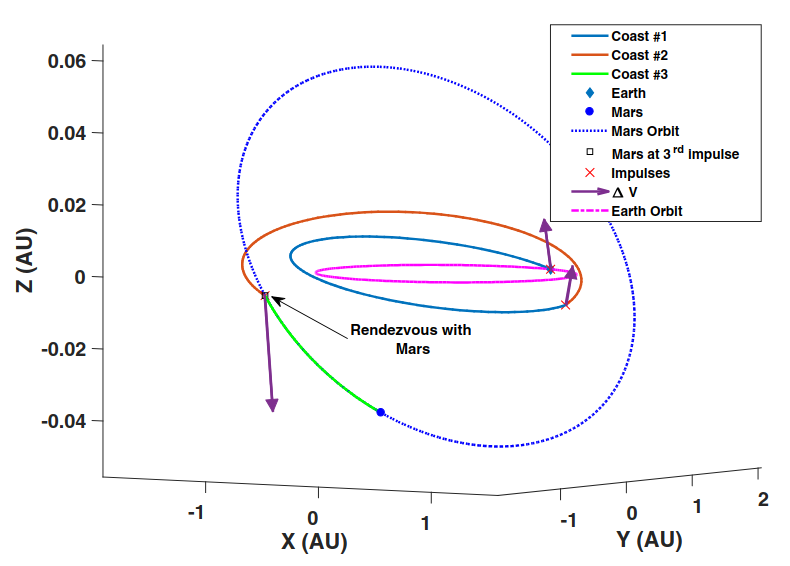
\includegraphics[width=0.6\textwidth]{img/impulsive_traj_from_how_many_impulses.png}
    \caption{illustration of impulsive transfer with Eart to Mars transfer in 3 impulses. Source: \cite{how_many_impulses}.}
    \label{fig:impulsive_maneuver_diagram}
\end{figure}

Tsiolkovsky's equation can be applied to all impulses, thus relating the final and initial masses with the total velocity change, which is the sum of all \(n\) burns executed during the transfer:
\begin{equation}
    m(t_f) = m(0) \exp{\left(-\frac{\sum_{i=1}^{n}\Delta v_i}{v_e}\right)}
\end{equation}

Since \(v_e\) and \(m(0)\) are not subject to optimization, the objective~\eqref{eq:max_final_mass} is equivalent to minimizing the sum of magnitudes of impulses used during the transfer:
\begin{equation}
    \min \sum_{i=1}^{n} \Delta v_i.
\end{equation}

Thus, in the impulsive case, the problem is \textit{independent of spacecraft mass}, and it can be eliminated from the state vector. However, the control trajectory \(\mathbf{\Gamma}(t)\) in the impulsive case is not a function, but a \textit{measure}. It therefore needs to be implemented not as a function of time, as usual in optimal control, but as magnitudes of discontinuities in the state trajectory. This introduces the number of allowed impulses as an optimization hyperparameter~\cite{optimal_impulsive_control}. To choose an optimal number of impulses, the theory of primer vectors (see ahead) can help determine the number of impulses needed~\cite{interactive_primer_vector}.

\subsubsection{Hohmann transfer}\label{sssec:hohmann}

\begin{figure}[htbp]
    \centering
    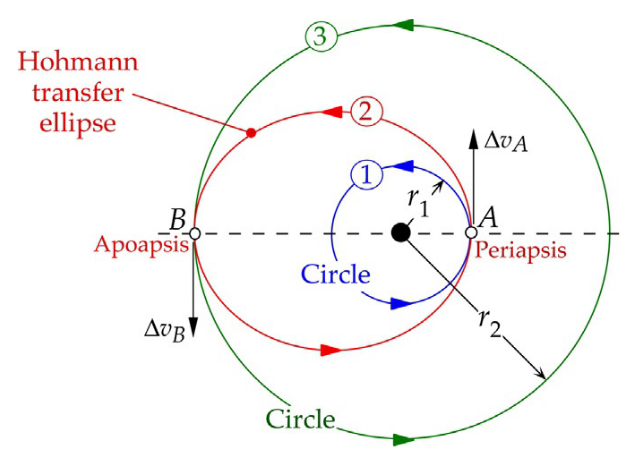
\includegraphics[width=0.6\textwidth]{img/hohmann_from_curtis.png}
    \caption{Hohmann transfer diagram. Source: \cite{curtis2015orbital}}
    \label{fig:hohmann_diagram}
\end{figure}

The prototypical orbital maneuver case is that of a two-impulse transfer between two coplanar circular orbits in Keplerian dynamics~\cite{chobotov}. The intermediate orbit, between the two impulses, is an ellipse that is tangent to both initial and final orbits, as can be seen in Figure~\ref{fig:hohmann_diagram}. This transfer has a known analytical optimal, which can be proven by several different methods. Some useful quantities relating to this transfer are given in the following. Given an initial circular orbit of semi-major axis \(a_1\) and a final circular orbit with semi-major axis \(a_2\), the total change in speed required is equal to~\cite{chobotov}:
\begin{equation}\label{eq:hohmann_deltav}
    \sum \lVert \Delta \mathbf{v} \rVert = \sqrt{\mu\left(\frac{2}{a_1}-\frac{2}{a_1+a_2}\right)} - \sqrt{\frac{\mu}{a_1}} + \sqrt{\frac{\mu}{a_2}} - \sqrt{\mu\left(\frac{2}{a_2}-\frac{2}{a_1+a_2}\right)}
\end{equation}

The transfer time is half of the transfer orbit's period. With \(t_H\) being the Hohmann transfer duration, is is given by~\cite{chobotov} 
\begin{equation}\label{eq:hohmann_time}
    t_H = \pi \sqrt{\frac{\left(\frac{a_1+a_2}{2}\right)^3}{\mu}}.
\end{equation}

% talk about stm
\section{Primer vector theory}
%redo for impulsive maneuvers: Hamiltonionan must be constant
%do for multiple models
The application of optimal control theory to orbital maneuvers dates back to the 1960s, with pioneering work by Lawden~\cite{Conway_2010}. In particular, he coined the term "primer vector"  as an analogy with the fact that the costate trajectory imposes a necessary condition for firing the engines, thus acting as a "primer". This theory is based on the indirect necessary conditions provided by the Hamiltonian formalism previously exposed, and is explored in~\citeonline{Conway_2010}. Here, the impulsive thrust case will be treated as a limiting case of finite thrust when \(\Gamma_{\max} \rightarrow \infty\). 

\subsection{Conservative Orbital model}

Firstly, a model where \(\ddot{\pos} = g(\pos) = \nabla \Phi(\pos)\), where \(\Phi(\pos)\) is a gravitational potential field, is considered. This type of model contains the two body approach as well as the J2 model. 

The acceleration due to the thrust \(\mathbf{\Gamma} \) can be split into its magnitude and direction as \(\mathbf{\Gamma} = \Gamma \hat{\mathbf{u}}\), \(\Gamma = \lVert \mathbf{\Gamma} \rVert\), \(\lVert \hat{\mathbf{u}} \rVert = 1\) so that the objective from Equation~\eqref{eq:obj_continuous_thrust} can be rewritten as
\begin{equation}
    \min_{\Gamma(t), \hat{\mathbf{u}}(t)} \int_0^{t_f} \Gamma dt
\end{equation}
and the Hamiltonian of the system is the given by
\begin{equation}
    H = \Gamma + \begin{bmatrix}
        \mathbf{\lambda}_r^T & \mathbf{\lambda}_v^T
    \end{bmatrix} \begin{bmatrix}
        \mathbf{v} \\ g(\mathbf{r}) + \Gamma \hat{\mathbf{u}}
    \end{bmatrix}
\end{equation}

The costate is subject to the adjoint equations given in block matrix form as
\begin{equation}\label{eq:lambda_dot_cons}
    \begin{bmatrix}
        \dot{\mathbf{\lambda}}_r \\ \dot{\mathbf{\lambda}}_v
    \end{bmatrix} = \begin{bmatrix}
        0_{3\times3} & -\left(\frac{\partial g(\mathbf{r})}{\partial \mathbf{r}}\right)^T \\
        -I_{3\times3} & 0
    \end{bmatrix} \begin{bmatrix}
        \mathbf{\lambda}_r \\ \mathbf{\lambda}_v
    \end{bmatrix}
\end{equation}
which is linear in the costate variables. For problems with final position and velocity constraints, no boundary conditions are given for the adjoint equations.

Rearranging the Hamiltonian to factor \(\Gamma \), 
\begin{equation}
    H = (1 + \mathbf{\lambda}_v^T \hat{\mathbf{u})} \Gamma + \mathbf{\lambda}_r^T \mathbf{v} + \mathbf{\lambda}_v^T g(\mathbf{r}).
\end{equation}

By applying Pontryagin's Minimum Principle, the thrust magnitude \(\Gamma\) is given piecewise by analyzing the sign of its coefficient:
\begin{equation}
    \Gamma = \begin{cases}
        \Gamma_{\max}&, 1+\mathbf{\lambda}_v^T \hat{\mathbf{u}} < 0 \\
        0&, 1 + \mathbf{\lambda}_v^T \hat{\mathbf{u}} > 0 \\
        \text{intermediate}&, \text{otherwise}
    \end{cases}
\end{equation}

%check what lawden has to say
The case where \(1 + \mathbf{\lambda}_v^T \hat{\mathbf{u}} = 0\) on a finite interval of time will not be considered here; these are \textit{singular arcs} and occur rarely~\cite{singular_arcs}. When \(\Gamma = \Gamma_{\max}\), its coefficient should be as negative as possible, which happens when \(\hat{\mathbf{u}}\) has the opposite direction to \(\mathbf{\lambda}_v\):
\begin{equation}
    \hat{\mathbf{u}} = - \frac{\mathbf{\lambda}_v}{\lVert \mathbf{\lambda}_v \rVert}.
\end{equation}

This direction, the \textit{optimal thrust direction} given by \(-\mathbf{\lambda}_v\) is what constitutes the primer vector \(\mathbf{p}\), which is defined as 
\begin{equation}\label{eq:p_lambda_v_cons}
    \mathbf{p} = -\mathbf{\lambda}_v.
\end{equation}

The engine firing conditions can be stated solely as a function of the primer vector as~\cite{Conway_2010}
\begin{equation}
    \Gamma = \begin{cases}
        \Gamma_{\max}&, \lVert \mathbf{p} \rVert > 1 \\
        0&, \lVert \mathbf{p} \rVert < 1 \\
        \text{intermediate}&, \text{otherwise}
    \end{cases}
\end{equation}

The impulsive thrust case is then found by letting \(\Gamma_{\max} \rightarrow \infty\), in which case the segments where \(\lVert \mathbf{p} \rVert > 1\) approach points, and the thrust cases become

\begin{equation}
    \Gamma = \begin{cases}
        0&, \lVert \mathbf{p} \rVert < 1 \\
        \Delta \vel \delta&, \lVert \mathbf{p} \rVert = 1 \\
    \end{cases},
\end{equation}
for some (possibly null) velocity increment \(\Delta \vel\)

Alternatively, one could reason about the constant value of the Hamiltonian which, from Equation~\eqref{eq:constant_hamilt}, is finite. Therefore, at the impulse instants, where \(\Gamma\) is unbounded, its coefficient \(1 + \lambda_v^T \hat{\uc}\) must be \(0\), leading to \(\hat{\uc} = -\lambda_v = \mathbf{p}\), and the condition \(\lVert \mathbf{p} \rVert = 1\).

The necessary conditions offered by primer vector theory for an impulsive maneuver scenario are~\cite{Conway_2010}:
\begin{enumerate}
    \item \(\mathbf{p}(t)\) and \(\dot{\mathbf{p}}(t)\) are continuous;
    \item \(\lVert \mathbf{p} \rVert \leq 1\);
    \item \(\mathbf{p} = \hat{\mathbf{u}}\) at the impulse instants, with the corollary that when an impulse happens, \(\lVert \mathbf{p} \rVert = 1\);
    \item \(\frac{d \lVert \mathbf{p} \rVert}{dt} = 0\) at impulses between the initial and final times (non-inclusive).
\end{enumerate}

In addition to these conditions for the optimal solution, variational calculus results can give some insight into how to change a suboptimal trajectory based on how those conditions are violated~\cite{Conway_2010}. For a maneuver with start time between times \(0\) and \(t_f\), these results can be enumerated:
\begin{enumerate}
    \item If the maneuver starts with an impulse (\(\lVert \mathbf{p}(0) \rVert = 1\)) and \(\partial_t \lVert \mathbf{p} \rVert \mid_{t=0} > 0\), adding an initial coast will lower the cost;
    \item If the maneuver ends with an impulse (\(\lVert \mathbf{p}(t_f) \rVert = 1\)) and \(\partial_t \lVert \mathbf{p} \rVert \mid_{t=0} < 0\), adding a final coast will lower the cost;
    \item If \(\lVert \mathbf{p}(t) \rVert > 1\) for some \(t \in [0, t_f]\), adding an impulse will lower the cost.
\end{enumerate}

\subsubsection{Primer vector calculation}\label{sssec:pv_calc_cons}

From Equations~\eqref{eq:lambda_dot_cons} and \eqref{eq:p_lambda_v_cons}, the primer vector differential equations are
\begin{equation}\label{eq:pdot_const}
    \begin{bmatrix}
        \dot{\mathbf{p}} \\ \ddot{\mathbf{p}}
    \end{bmatrix} = \begin{bmatrix}
        \mathbf{0}_3 & \mathbf{I}_3 \\
        \left[\frac{\partial g}{\partial \pos}\right]^T & \mathbf{0}_3
    \end{bmatrix} \begin{bmatrix}
        \mathbf{p} \\ \dot{\mathbf{p}}
    \end{bmatrix} = \mathbf{A}_p \begin{bmatrix}
        \mathbf{p} \\ \dot{\mathbf{p}}
    \end{bmatrix}
\end{equation}

Since Equation~\eqref{eq:pdot_const} is linear on the variables, it admits a solution through the form of a primer vector transition matrix (PVTM) \(\mathbf{\Phi}_p(t - t_0)\) such that
\begin{equation}
    \begin{bmatrix}
        \mathbf{p}(t) \\ \dot{\mathbf{p}}(t)
    \end{bmatrix} = \mathbf{\Phi}_p(t - t_0) \begin{bmatrix}
        \mathbf{p}(t_0) \\ \dot{\mathbf{p}}(t_0)
    \end{bmatrix}.
\end{equation}
However, since \(g = \nabla \Phi = \left(\frac{\partial \Phi}{\partial \pos}\right)^T\), \(\left[\frac{\partial g}{\partial \pos}\right]\) is actually the Hessian matrix of the potential field, which is symmetric. Therefore, the primer vector is subject to the same differential equation as the STM in Equation~\eqref{eq:STM_r_v}, and Equation~\eqref{eq:remark_STM} can be used to equate the PVTM to the STM:
\begin{equation}
    \mathbf{\Phi}_p(t - t_0) = \mathbf{\Phi}_\delta(t - t_0) = \frac{\partial \x(t)}{\partial \x(t_0)}.
\end{equation}

This way of computing \(\mathbf{\Phi}_p(t - t_0)\) will be termed the STM method for primer vector calculation, and is valid for all conservative force models. For the two body model in particular, a closed form for \(\mathbf{\Phi}_p(t-t_0)\) exists~\cite{glandorf_transition_matrix}. 

Computing the primer vector trajectory is done piecewise on coasting arcs between two consecutive impulses, since the primer vector is known at impulse times. Since \(\mathbf{p}\) is known at both ends, but not \(\dot{\mathbf{p}}\), this configures a linear TPBVP\@. For two consecutive impulses, \(\Delta v_1\) at time \(t_1\) and \(\Delta v_2\) at time \(t_2\), the primer vector values are given by:
\begin{align}\label{eq:pv_deltav}
    \mathbf{p}(t_1) &= \frac{\Delta \mathbf{v}_1}{\lVert \Delta \mathbf{v}_1 \rVert} \\
    \mathbf{p}(t_2) &= \frac{\Delta \mathbf{v}_1}{\lVert \Delta \mathbf{v}_2 \rVert}
\end{align}

The state transition between these two instants can be stated as
\begin{equation}
    \begin{bmatrix}
        \mathbf{p}(t_2) \\ \dot{\mathbf{p}}(t_2)
    \end{bmatrix} = \mathbf{\Phi}_p(t_2 - t_1) \begin{bmatrix}
        \mathbf{p}(t_1) \\ \dot{\mathbf{p}}(t_1)
    \end{bmatrix} = \begin{bmatrix}
        \mathbf{M}(t_2-t_1) & \mathbf{N}(t_2-t_1) \\ \mathbf{S}(t_2-t_1) & \mathbf{T}(t_2-t_1)
    \end{bmatrix} \begin{bmatrix}
        \mathbf{p}(t_1) \\ \dot{\mathbf{p}}(t_1)
    \end{bmatrix}
\end{equation}
where \(\mathbf{M}\), \(\mathbf{N}\), \(\mathbf{S}\) and \(\mathbf{T}\) are square matrices. From now on the times shall be denoted as indices for conciseness. If \(\mathbf{p}\) and \(\dot{\mathbf{p}}\) are known for a certain time, the entire trajectory can be found. It is easy to isolate \(\dot{\mathbf{p}}_1 = \dot{\mathbf{p}}(t_1)\):
\begin{equation}
    \dot{\mathbf{p}}_1 = \mathbf{N}^{-1}_{21} \left(\mathbf{p}_2 - \mathbf{M}_{21}\mathbf{p}_1\right).
\end{equation}

\(\mathbf{N}_{21}\) is invertible except for isolated values of \(t\)~\cite{Conway_2010}; in these cases, the primer vector trajectory is assumed to lie in the orbital plane, spanned by \(\begin{bmatrix}
    \mathbf{r}_1 & \mathbf{v}_1
\end{bmatrix}\). Thus, for singular \(N\),
\begin{equation}\label{eq:pdot1_singular}
    \dot{\mathbf{p}}_1 = \begin{bmatrix}
        \mathbf{r}_1 & \mathbf{v}_1
    \end{bmatrix} (\mathbf{N}_{21} \begin{bmatrix}
        \mathbf{r}_1 & \mathbf{v}_1
    \end{bmatrix})^\dagger \left(\mathbf{p}_2 - \mathbf{M}_{21}\mathbf{p}_1\right)
\end{equation}
where \(A^\dagger\) denotes the pseudo-inverse of a rectangular matrix.

% Some typical primer vector magnitude trajectories are given in Figure~\ref{fig:primer_trajectory_example}. 

% Notice how in Figure~\ref{fig:primer_trajectory_example}, the first trajectory satisfies all necessary conditions, the second one violates condition 2, and the third one violates condition one. How to exploit necessary condition violation for improving trajectories shall be discussed in future work.

% \begin{figure}[htbp]
%     \centering
%     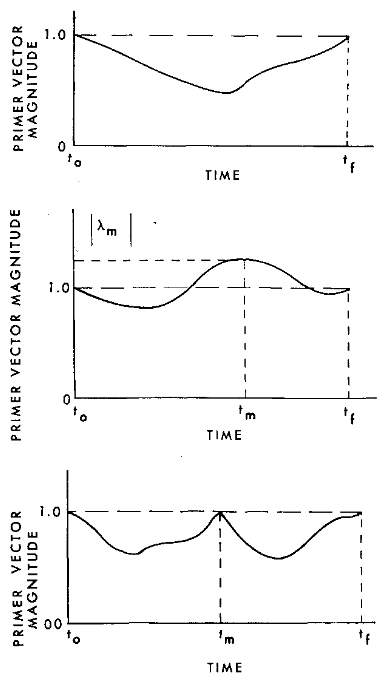
\includegraphics[width=0.3\textwidth]{img/primer_vector_history_from_jezewsky.png}
%     \caption{Typical primer vector trajectories. Source: \cite{efficient_n_impulse}.}
%     \label{fig:primer_trajectory_example}
% \end{figure}

\subsection{Non-conservative Orbital model}

Here, the model considered has a conservative part \(g(\pos)\) and a non-conservative part \(d(\pos, \vel)\), representing drag, or other non-conservative forces, such that \(\ddot{\pos} = g(\pos) + d(\pos, \vel)\).

The Hamiltonian of the system is the given by
\begin{equation}
    H = \Gamma + \begin{bmatrix}
        \mathbf{\lambda}_r^T & \mathbf{\lambda}_v^T
    \end{bmatrix} \begin{bmatrix}
        \mathbf{v} \\ g(\mathbf{r}) + d(\pos, \vel) + \Gamma \hat{\mathbf{u}}
    \end{bmatrix}
\end{equation}

The costate is subject to the adjoint equations given in block matrix form as
\begin{equation}\label{eq:lambda_dot_ncon}
    \begin{bmatrix}
        \dot{\mathbf{\lambda}}_r \\ \dot{\mathbf{\lambda}}_v
    \end{bmatrix} = \begin{bmatrix}
        0_{3\times3} & -\left[\frac{\partial }{\partial \mathbf{r}}\big(g(\mathbf{r}) + d(\pos, \vel)\big)\right]^T \\
        -I_{3\times3} & -\left(\frac{\partial d(\pos, \vel)}{\partial \vel}\right)^T 
    \end{bmatrix} \begin{bmatrix}
        \mathbf{\lambda}_r \\ \mathbf{\lambda}_v
    \end{bmatrix}.
\end{equation}

Rearranging the Hamiltonian to factor \(\Gamma \), 
\begin{equation}
    H = (1 + \mathbf{\lambda}_v^T \hat{\mathbf{u}}) \Gamma + \mathbf{\lambda}_r^T \mathbf{v} + \mathbf{\lambda}_v^T (g(\mathbf{r}) + d(\pos, \vel)).
\end{equation}

By similar reasoning to the conservative case, \(\mathbf{p} = - \lambda_v\), with the same necessary conditions. 

\subsubsection{Primer Vector calculation}\label{sssec:pv_calc_ncon}

The primer vector differential equation is the main difference of the non-conservative case w.r.t. the conservative case. It can be found from Equation~\eqref{eq:lambda_dot_ncon}:

\begin{equation}\label{eq:pdot_ncon}
    \begin{bmatrix}
        \dot{\mathbf{p}} \\ \ddot{\mathbf{p}}
    \end{bmatrix} = \begin{bmatrix}
        \mathbf{0}_3 & \mathbf{I}_3 \\
        \left[\frac{\partial }{\partial \mathbf{r}}\big(g(\mathbf{r}) + d(\pos, \vel)\big)\right]^T & -\left(\frac{\partial d(\pos, \vel)}{\partial \vel}\right)^T
    \end{bmatrix} \begin{bmatrix}
        \mathbf{p} \\ \dot{\mathbf{p}}
    \end{bmatrix} = \mathbf{A}_p \begin{bmatrix}
        \mathbf{p} \\ \dot{\mathbf{p}}
    \end{bmatrix}.
\end{equation}

Save some very particular non-conservative force models, the non-conservative primer vector dynamics in Equation~\eqref{eq:pdot_ncon} is \textbf{not} equal to the non-conservative variational perturbation differential equation, which disallows the STM method from being used. However, it remains a linear differential equation with transition matrix \(\mathbf{\Phi}_p(t - t_0)\) subject to 
\begin{equation}
    \begin{cases}
        \dot{\mathbf{\Phi}_p} = \mathbf{A}_p(\pos, \vel) \mathbf{\Phi}_p \\
        \mathbf{\Phi}_p(0) = \mathbf{0}_6
    \end{cases},
\end{equation}
which allows for the solution of a linear TPBVP as described in Equations~\eqref{eq:pv_deltav}-\eqref{eq:pdot1_singular}.

\subsection{Primer vector theory summary}

method of calculation x model

necessary conditions